\section{Controlling}

The main task of the project requires the robot to move with the highest possible speed.
On the other hand the robot should be able to move at a speed that induces as little drift as possible and reduces the risk of errors when hitting an obstacle.
And lastly, the vision would have to identify objects from further away, increasing the difficulty of implementation and recognition.
Thus, a balance in the velocities have to be found.\\

The implemented controllers consisted of a forward movement controller, a turn controller and a wall alignment controller.
By embedding them in an adapter pattern it was possible to render their usage very versatile (see figure \ref{fig:arch_controller}).
Every controller inherited hereby a controller base which defined an interface that updated the logic and returned a Twist
(A Twist is one of many ros pre-baked data structures that can be sent as a message. 
It stores a position and a rotation). 
The adapter combines all received Twists to one Twist, entrusting that no contradictions occur.
A top logic has to ensure that the right controllers are activated and deactivated.\\

Due to internal motor difference, it is not sufficient to control the motors directly.
Otherwise the robot would move in an arch, one motor rotating slower than the other.
To compensate for that and to also be able to input linear and angular velocities, a PID controller was used. 
This enabled the robot to drive in a stable straight line.

The motors itself have a static resistance, that initially had to be overcome whenever a control signal was sent.
These static resistances could be described by a constant $K_{power}$, that were added to the result of the PID results.
As soon as the static resistance has been overcome and the motor is rotating, the constant $K_{power}$ can be reduced to a value that sustains rotation: $K_{sustain}$.
This behavior results in a spiked motor control output as can be seen in figure \ref{fig:pwm_spiker}.
Although movement without spiking would not be a problem due to the accumulating behavior of the PID controller, it ensures a very responsive controlling.

\begin{figure}[h]
\begin{center}
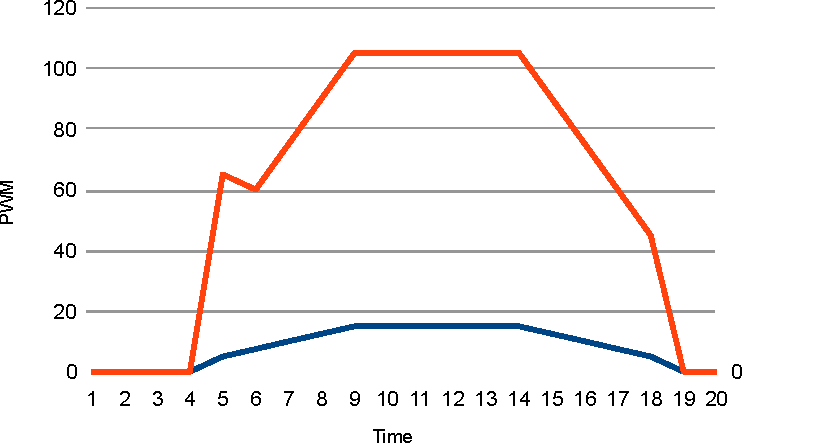
\includegraphics[width=0.5\textwidth]{figures/pwm_spike.pdf}
\end{center}
\caption{PWM Spiking for initial motor rotation attempt}
\label{fig:pwm_spiker}
\end{figure}